\chapter{Vyčítaná Wireless M-Bus zařízení}

Pro účely testování komunikace bylo využito několik typů dostupných zařízení:
\begin{itemize}
	\item modul pro vodoměry Bonega \cite{BonegaCidlo},
	\item Pikkerton \colorbox[rgb]{0,1,0}{upřesnit co to je, pripadne otestovat cteni.}
	\item pokojové čidlo teploty a vlhkosti Weptech OMST-868A \cite{WeptechCidlo},
	\item ZPA. \colorbox[rgb]{0,1,0}{upřesnit co to je, pripadne doplnit specifikaci.}
\end{itemize}

%%%%%%%%%%%%%%%%%%%%%%%%%%%%%%%%%%%%%%%%%%%%%%%%%%%%%%%%%%%%%%%%%%%%%%%%%%%%%%%%%%%%%%%%%%%%%%%%%%%%%%%%%%%%%%%%%%%%%%%%%%%%%%%%%%%%%%%%%
%%%%%%%%%%%%%%%%%%%%%%%%%%%%%%%%%%%%%%%%%%%%%%%%%%%%%%%%%%%%%%%%%%%%%%%%%%%%%%%%%%%%%%%%%%%%%%%%%%%%%%%%%%%%%%%%%%%%%%%%%%%%%%%%%%%%%%%%%
	

	\section{Bonega}

Modul Bonega je bezdrátové čidlo podporující protokol Wireless M-Bus. Jedná se o samostatné zařízení, které je určené pro montáž na vodoměry Bonega. Na řadu vodoměrů podporujících tento modul je možná i dodatečná montáž. Elektronická část modulu slouží současně pro vyčítání dvou vodoměrů, na teplou i studenou vodu.
	
	 \begin{figure}[!h]
  \begin{center}
    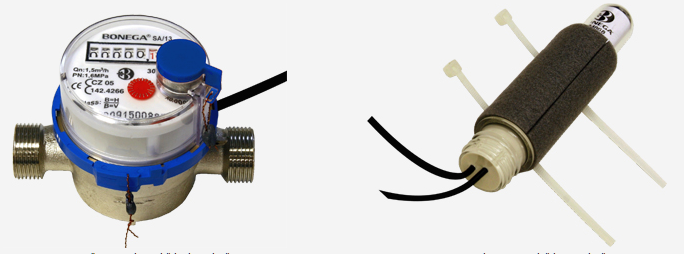
\includegraphics[scale=0.70]{obrazky/bonega_fotky}
  \end{center}
  \caption{Bezdrátový modul Bonega \cite{BonegaCidlo}}
\end{figure}


\subsubsection{Parametry modulu}
\begin{itemize}
	\item Rozsah měření: 0 až 65536 m\textsuperscript{2}.
	\item Přesnost měření: ± 1 litr.
	\item Maximální detekovatelný průtok: 6 m\textsuperscript{3}/hod.
	\item Mód přenosu: T1.
	\item Stupeň krytí: IP64.
	\item Interval přenosu: 20-24 sekund v odpočtovém období (od 1.11. do 15.1.)
	\item Interval přenosu: 4 minuty mimo odpočtové období.
	\item Šifrování přenosu: AES-128 mód 5.
	\item Napájení: integrovaná baterie.
	\item Výdrž baterie: až 12 let.
\end{itemize}


\subsubsection{Formát telegramu}
Zařízení vysílá postupně dva telegramy, s rozlišením šestým bajtem adresy zařízení, jeden pro vodoměr teplé vody a druhý pro vodoměr studené vody.
Telegram má specifickou základní strukturu popsanou v Tab\ref{TabulkaTelegram2} \cite{BonegaCidlo}:

\begin{table}[!ht]
\centering
\caption{Telegram z modulu Bonega \cite{BonegaCidlo}}
\resizebox{\textwidth}{!}{%
\label{TabulkaTelegram2}
\begin{tabular}{|c|l|c|}
\hline
\textbf{POLE}      & \textbf{POPIS}            & \textbf{HODNOTA} \\ \hline
L-Field            & Délka telegramu                                & 1Eh              \\ \hline
C-Field            & Typ telegramu                                  & 44h              \\ \hline
M-Field            & Výrobce zařízení                               & B0h              \\ \hline
M-Field            & Výrobce zařízení                               & 5Ch              \\ \hline
A-Field            & Sériové číslo                                  & 11h              \\ \hline
A-Field            & Sériové číslo                                  & 47h              \\ \hline
A-Field            & Sériové číslo                                  & 15h              \\ \hline
A-Field            & Sériové číslo                                  & 08h              \\ \hline
A-Field            & Verze zařízení                                 & 01h              \\ \hline
A-Field            & Typ zařízení                                   & 1Bh              \\ \hline
Ci-pole            & Odpověd od zařízení                            & 7Ah              \\ \hline
Access Number      & Číslo přístupu                                 & 41h              \\ \hline
Status             & Status zařízení                                & 00h              \\ \hline
Signature field 	 & Konfigurační řetězec AES                       & 00h              \\ \hline
Signature field    & Konfigurační řetězec AES                       & 00h              \\ \hline
Data						   & Ověření AES                                    & 2Fh              \\ \hline
Data						   & Ověření AES                                    & 2Fh              \\ \hline
Data               & DIF: 2 cifry BCD (určení formátu průtoku)      & 04h              \\ \hline
Data               & VIF: Objemový průtok v m krychlových na mínus první & 13h         \\ \hline
Data               & Hodnota průtoku                               & 99h               \\ \hline
Data               & Hodnota průtoku                               & 99h               \\ \hline
Data               & Hodnota průtoku                               & 99h               \\ \hline
Data               & Hodnota průtoku                               & 99h               \\ \hline
Data               & DIF: 2 cifry BCD (určení formátu času)         & 6Dh              \\ \hline
Data               & DIF: 2 cifry BCD                               & 6Dh              \\ \hline
Data               & Čas odeslání měření                           & 99h               \\ \hline
Data               & Čas odeslání měření                           & 99h               \\ \hline
Data               & Čas odeslání měření                           & 99h               \\ \hline
Data               & Čas odeslání měření                           & 99h               \\ \hline	
Data						   & Ověření AES                                    & 2Fh              \\ \hline
Data						   & Ověření AES                                    & 2Fh              \\ \hline

\end{tabular}}
\end{table}

\newpage{}

Modul Bonega pracuje pouze v režimu šifrování přenášenných dat pomocí AES128 mód 5. Při přenosu je tedy celá sekce data šifrována, telegram popsaný v tabulce \ref{TabulkaTelegram2} je popisován po dešifrování.

Některé z položek je potřeba blíže vysvětlit:

\begin{itemize}
	\item Access number - Toto číslo se s každým požadavkem zvýší o hodnotu 1.
	\item Status - V případě úspěšného přenosu je zde uložena nula, v opačném případě je zde uložena logická jednička a nastal tedy chybový stav 'únik vody' nebo 'vybitá baterie'.
	\item Signature field - V případě zapnutého šifrovaní, první bajt obsahuje počet zašifrovaných bloků, obsah telegarmu a inkrement. Druhý bajt obsahuje záznam o obousměrnosti, dostupnosti, synchronizaci a šifrování. Pokud je šifrování zapnuto, je nastaven mód 5, v opačném případě jsou oba bajty nulové.
	\item Hodnota průtoku - aktuální hodnota průtoku je zde vyjádřena čtyři hexadecimálními bajty v LSB pořadí.
	\item Čas odeslání měření - \colorbox[rgb]{0,1,0}{Dopsat až to bude umět aplikace. Viz PPT od PM}
\end{itemize}




%%%%%%%%%%%%%%%%%%%%%%%%%%%%%%%%%%%%%%%%%%%%%%%%%%%%%%%%%%%%%%%%%%%%%%%%%%%%%%%%%%%%%%%%%%%%%%%%%%%%%%%%%%%%%%%%%%%%%%%%%%%%%%%%%%%%%%%%%
%%%%%%%%%%%%%%%%%%%%%%%%%%%%%%%%%%%%%%%%%%%%%%%%%%%%%%%%%%%%%%%%%%%%%%%%%%%%%%%%%%%%%%%%%%%%%%%%%%%%%%%%%%%%%%%%%%%%%%%%%%%%%%%%%%%%%%%%%
	
		\section{Pikkerton}


\colorbox[rgb]{0,1,0}{Budeme vyčítat nějaké zařízení Pikkerton?}

\colorbox[rgb]{0,1,0}{Aplikace to má implementované, ale potřebuji test, je tam toho celkem hodně.}
	
	
	%%%%%%%%%%%%%%%%%%%%%%%%%%%%%%%%%%%%%%%%%%%%%%%%%%%%%%%%%%%%%%%%%%%%%%%%%%%%%%%%%%%%%%%%%%%%%%%%%%%%%%%%%%%%%%%%%%%%%%%%%%%%%%%%%%%%%%%%%
%%%%%%%%%%%%%%%%%%%%%%%%%%%%%%%%%%%%%%%%%%%%%%%%%%%%%%%%%%%%%%%%%%%%%%%%%%%%%%%%%%%%%%%%%%%%%%%%%%%%%%%%%%%%%%%%%%%%%%%%%%%%%%%%%%%%%%%%%
	
	
	\section{Weptech OMST-868A}
	
	Weptech OMST-868A je teplotní a vlhkostní čidlo podporující protokol Wireless M-Bus. Je určeno pro vnitřní využití a proto je dodáváno v pouzdře určeném pro montáž na zeď.
	
	 \begin{figure}[!h]
  \begin{center}
    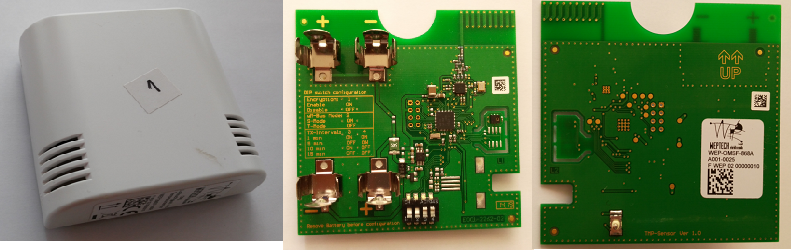
\includegraphics[scale=0.70]{obrazky/weptech_fotky}
  \end{center}
  \caption{Čidlo Weptech OMST-868A \cite{WeptechCidlo}}
\end{figure}


\subsubsection{Parametry čidla}
\begin{itemize}
	\item Rozsah měření vlhkosti: 20 až 80\%.
	\item Přesnost měření vlhkosti: ± 2\%.
	\item Rozsah měření teploty: -10°C až 55°C.
	\item Přesnost měření teploty: ± 0,3°C.
	\item Teplotní hystereze: 0,1°C.
	\item Mód přenosu: S nebo T.
	\item Interval přenosu: konfiugurovatelný v rozsahu 5 sekund až 24 hodin.
	\item Šifrování přenosu: volitelný AES-128 mód 5.
	\item Napájení: 2 x AA baterie.
	\item Výdrž baterie: dle módu a intervalu přenosu až 10 let.
\end{itemize}


\subsubsection{Formát telegramu}

Telegram má specifickou základní strukturu popsanou v Tab\ref{TabulkaTelegram} \cite{WeptechCidlo}:

\begin{table}[!ht]
\centering
\caption{Telegram ze zařízení Weptech 868A \cite{WeptechCidlo}}
\label{TabulkaTelegram}
\resizebox{\textwidth}{!}{%
\begin{tabular}{|c|l|c|}
\hline
\textbf{POLE}      & \textbf{POPIS}            & \textbf{HODNOTA} \\ \hline
L-Field            & Délka telegramu                                & 1Eh              \\ \hline
C-Field            & Typ telegramu                                  & 44h              \\ \hline
M-Field            & Výrobce zařízení                               & B0h              \\ \hline
M-Field            & Výrobce zařízení                               & 5Ch              \\ \hline
A-Field            & Sériové číslo                                  & 11h              \\ \hline
A-Field            & Sériové číslo                                  & 47h              \\ \hline
A-Field            & Sériové číslo                                  & 15h              \\ \hline
A-Field            & Sériové číslo                                  & 08h              \\ \hline
A-Field            & Verze zařízení                                 & 01h              \\ \hline
A-Field            & Typ zařízení                                   & 1Bh              \\ \hline
Ci-pole            & Odpověd od zařízení                            & 7Ah              \\ \hline
Access Number      & Číslo přístupu                                 & 41h              \\ \hline
Status             & Status zařízení                                & 00h              \\ \hline
Configuration word & Konfigurační řetězec AES                       & 00h              \\ \hline
Configuration word & Konfigurační řetězec AES                       & 00h              \\ \hline
AES verification   & Ověření AES                                  & 2Fh              \\ \hline
AES verification   & Ověření AES                                  & 2Fh              \\ \hline
DR1                & DIF: 4 cifry BCD                               & 0Ah              \\ \hline
DR1                & VIF: teplota ve stupních Celsia na mínus první & 66h              \\ \hline
DR1                & Hodnota teploty                                & 99h              \\ \hline
DR1                & Hodnota teploty                                & 01h              \\ \hline
DR2                & DIF: 4 cifry BCD                               & 0Ah              \\ \hline
DR2                & VIF: První rozšiřovací tabulka                 & FBh              \\ \hline
DR2                & VIFE: vlhkost procentech na mínus první        & 1Ah              \\ \hline
DR2                & Hodnota relativní vlhkosti                               & 93h              \\ \hline
DR2                & Hodnota relativní vlhkosti                               & 02h              \\ \hline
DR3                & DIF: 16bit integer/binary                      & 02h              \\ \hline
DR3                & VIF: Druhá rozšiřovací tabulka                 & FDh              \\ \hline
DR3                & VIFE0: Chybové stavy                           & 97h              \\ \hline
DR3                & VIFE1: Norma 																	& 1Dh              \\ \hline
DR3                & Příznak sabotáže                               & 00h              \\ \hline
DR3                & Příznak vybité baterie                         & 00h              \\ \hline
Fill               & Výplňové byty (13x)                                 & 2Fh              \\ \hline

\end{tabular}}
\end{table}

\newpage{}

Některé z položek je potřeba blíže vysvětlit:

\begin{itemize}
	\item Access number - Toto číslo se s každým požadavkem zvýší o hodnotu 1.
	\item Status - V případě úspěšného přenosu je zde uložena nula, v opačném případě je zde uložena logická jednička a nastal tedy chybový stav 'sabotáž' nebo 'vybitá baterie'.
	\item Configuration word - V případě zapnutého šifrovaní, první bajt obsahuje počet zašifrovaných bloků, obsah telegarmu a inkrement. Druhý bajt obsahuje záznam o obousměrnosti, dostupnosti, synchronizaci a šifrování. Pokud je šifrování zapnuto, je nastaven mód 5, v opačném případě jsou oba bajty nulové.
	\item Příznak sabotáže čidla - Pokud čidlo pomocí integrovaného spínače detekuje uvolnění krytu z montážní desky, pošle výstrahu přes rádio do přijímače, tedy změní pro nejbližší a všechny následující vysílání tamper bit v telegramu. Tento bit slouží jako ochrana před neoprávněnou manipulací s čidlem a může být vymazán pouze restartem zařízení. Tedy vyjmutím starých baterií, ponecháním zařízení několik minut bez napájení, aby došlo k vybití všech kondenzátorů a následným vložením baterií.
\item Příznak vybité baterie - Pokud elektronika v čidlu vyhodnotí úroveň nabití baterie jako nedostatečnou, nastaví bit vybití baterie do sekce chyb v telegramu. Tento bit ošetřuje stavy, kdy nedostatečně nabité baterie způsobí příliš velký rozptyl naměřených hodnot, v krajních případech i mimo měřící rozsah čidla. Tento bit může být vymazán také pouze restartem zařízení, jako v předchozím případě.
\item Položky hodnota teploty, hodnota vlhkosti, výrobce zařízení a sériové číslo jsou uloženy v kódování big-endian, tedy na paměťové místo s nejnižší adresou se uloží nejvíce významný bajt a za něj se ukládají ostatní bajty až po nejméně významný bajt na konci. Uživatelská hodnota se tedy vyčítá pozpátku pod jednotlivých bajtech.
\item Telegram je ukončen 13 výplňovými bajty, které nenesou žádnou informaci.
\end{itemize}


\subsubsection{Nastavení čidla}
Čidlo má k dispozici několik nastavení. Některé z nich lze nastavit pomocí čtyř přepínačů DIP na desce plošných spojů.
První přepínač zapíná AES-128 šifrování, druhý přepínač přepíná mezí módem vysílání S (poloha ON) a módem T (poloha OFF), třetí a čtvrtý přpínač určují interval zasílání telegramu, jejich nastavení shrnuje Tab.\ref{TablukaDIP}.

\newpage{}

\begin{table}[!ht]
\centering
\caption{Konfigurace intervalu zasílání pomocí DIP přepínače \cite{WeptechCidlo}}
\label{TablukaDIP}
\begin{tabular}{|c|c|c|}
\hline
\textbf{Interval zasílání} & DIP 3 & DIP 4 \\ \hline
1 minuta & ON & ON \\ \hline
5 minut & OFF & ON \\ \hline
10 minut & ON & OFF \\ \hline
15 minut & OFF & OFF \\ \hline
\end{tabular}
\end{table}

Jiné mohou být nastaveny pouze během výroby daného setu, a to do příslušnch továrních nastavení, či uživatelsky vyžádaných nastavení, viz Tab. \ref{TablukaSETUP}.

\begin{table}[!ht]
\centering
\caption{Přehled nastavení čidla \cite{WeptechCidlo}}
\label{TablukaSETUP}
\begin{tabular}{|c|l|c|}
\hline
\textbf{Parametr} & \multicolumn{1}{c|}{\textbf{Popis}} & \textbf{\begin{tabular}[c]{@{}c@{}}DIP \\ přepínač\end{tabular}} \\ \hline
AES enable & \begin{tabular}[c]{@{}l@{}}Možnost zapnutí či vypnutí šifrování \\ přenášených dat.\end{tabular} & 1 \\ \hline
%AES key & \begin{tabular}[c]{@{}l@{}}AES klíč je zapsán při výrobě zařízení, \\ nelze ho uživatelsky měnit. Hodnota \\ klíče je 00 01 02 03 04 05 06 07 08 \\ 09 0A 0B 0C 0D 0E 0F.\end{tabular} &  \\ \hline
wM-Bus mode & \begin{tabular}[c]{@{}l@{}}Implementovány jsou módy S1-m \\ a T1. Ostatní módy lze nastavit\\ pouze při tovární výrobě.\end{tabular} & 2 \\ \hline
Transmission interval & \begin{tabular}[c]{@{}l@{}}Interval je výrobcem konfigurovatelný \\ v intervalu 2 až 65534 sekund. \\ Předvolby (60s, 300s, 600s, 900s) \\ jsou uživatelsky nastavitelné pomocí \\ DIP přepínače.\end{tabular} & 3 a 4 \\ \hline
%Address & \begin{tabular}[c]{@{}l@{}}Adresa zařízení je výrobcem udaná \\ hodnota, obsahující identifikaci \\ výrobce „WEP“, sériového číslo čidla, \\ verzi zařízení (1) a typ \\ zařízení (1Bh - pokojové čidlo)\end{tabular} &  \\ \hline
%Tamper & \begin{tabular}[c]{@{}l@{}}Odezva od čidla pro otevření \\ boxu může být povolena či \\ zakázána, samotné zařízení \\ existuje i ve verzích bez \\ tohoto čidla.\end{tabular} & \multicolumn{1}{l|}{} \\ \hline
%Config & \begin{tabular}[c]{@{}l@{}}Změna nastavení pomocí DIP \\ přepínače může být povolena \\ či zakázána, samotné zařízení \\ existuje i ve verzích bez\\  tohoto přepínače.\end{tabular} & \multicolumn{1}{l|}{} \\ \hline
\end{tabular}
\end{table}


%%%%%%%%%%%%%%%%%%%%%%%%%%%%%%%%%%%%%%%%%%%%%%%%%%%%%%%%%%%%%%%%%%%%%%%%%%%%%%%%%%%%%%%%%%%%%%%%%%%%%%%%%%%%%%%%%%%%%%%%%%%%%%%%%%%%%%%%%
%%%%%%%%%%%%%%%%%%%%%%%%%%%%%%%%%%%%%%%%%%%%%%%%%%%%%%%%%%%%%%%%%%%%%%%%%%%%%%%%%%%%%%%%%%%%%%%%%%%%%%%%%%%%%%%%%%%%%%%%%%%%%%%%%%%%%%%%%


	\section{ZPA}
	\colorbox[rgb]{0,1,0}{Budeme vyčítat nějaký elektroměr ZPA?}
	
